
\section{Definitions and intuition}
Probability is a measure of:
\begin{itemize}
    \item Our certainty or belief that a statement is true. My belief could be different than yours;
    \item How frequently an event will occur.
\end{itemize}
\begin{mydefinition}[Random experiment]
        A \emph{random experiment} is an experiment (or a physical process) whose outcome is not certain but all of its possible outcomes are known and predictable in advance.        

        A random experiment is modeled as a probability space (check Definition~\ref{def: proability space}).
\end{mydefinition}
\begin{mydefinition}[Sample space $S$]
    The \emph{sample space} $S$ is the set of \emph{all} possible \emph{outcomes}.
\end{mydefinition}

\begin{mydefinition}[Event]
    An \emph{event} $A$ is a \emph{subset} of $S$. That is, $A\subseteq S$. It's NOT an element of $S$! It is rather an element of the power set $\pSet_{S}$ (Definition~\ref{def: power set}).

    Thus, an event $A$ is a \emph{set} of outcomes. 
\end{mydefinition}
\begin{mydefinition}[Power set of $S$]
    \label{def: power set}
    The \emph{power set} of the sample space $S$ is the set containing all subsets of a set $S$. It's denoted by $\pSet_{S}$, or simply $\pSet$.
    \thline
    \begin{itemize}
        \item $\pSet_{S}$ is the set of all events.
        \item $\varnothing \subseteq S$: Impossible event.
        \item $S \subseteq S$: Certain event.
    \end{itemize}
\end{mydefinition}
\begin{example}[Flipping a coin]
    Flipping a coin \emph{once} has the sample space
    \begin{align}
        S &= \{H, T\},
    \end{align}
    $H$ and $T$ are all the possible \emph{outcomes} (NOT events) of the sample space $S$. The power set is thus given by
    \begin{align}
        \pSet_{S} &= \left\{\{\varnothing\}, \{H\}, \{T\}, \{H,T\}\right\}.
    \end{align}
    Note that the last element of $\pSet_{S}$, $\{H,T\}$ is the sample space and it is thus a \emph{certain} event. 
    \triqed
\end{example}

\begin{example}[Number of occurences]
    Relative frequency interpretation of probability (which is very intuitive).
    Say a random experiment gives an outcome $a$ in an event $A$ (i.e., $a\in A\subseteq S$) from the sample space. Repeat the experiment $N$ times. Then, define the number of occurrences of event $A$ after repeating the experiment $N$ times by
    \begin{align}
        n(A,N) &= \text{\# of times that $A$ happens}.
    \end{align}
    Note that ``\# of times that $A$ happens'' implies that the outcome $a_{k}$ of experiment $k$ belongs to the event $A$. That is, $a_{k}\in A$.
    Then, 
    \begin{align}
        \underbrace{\lim_{N\rightarrow\infty} \f{n(A,N)}{N}}_{\text{Probability of event $A$.}} = \text{constant}.
    \end{align}
    \triqed
\end{example}

\begin{figure}[h]
    \centering
    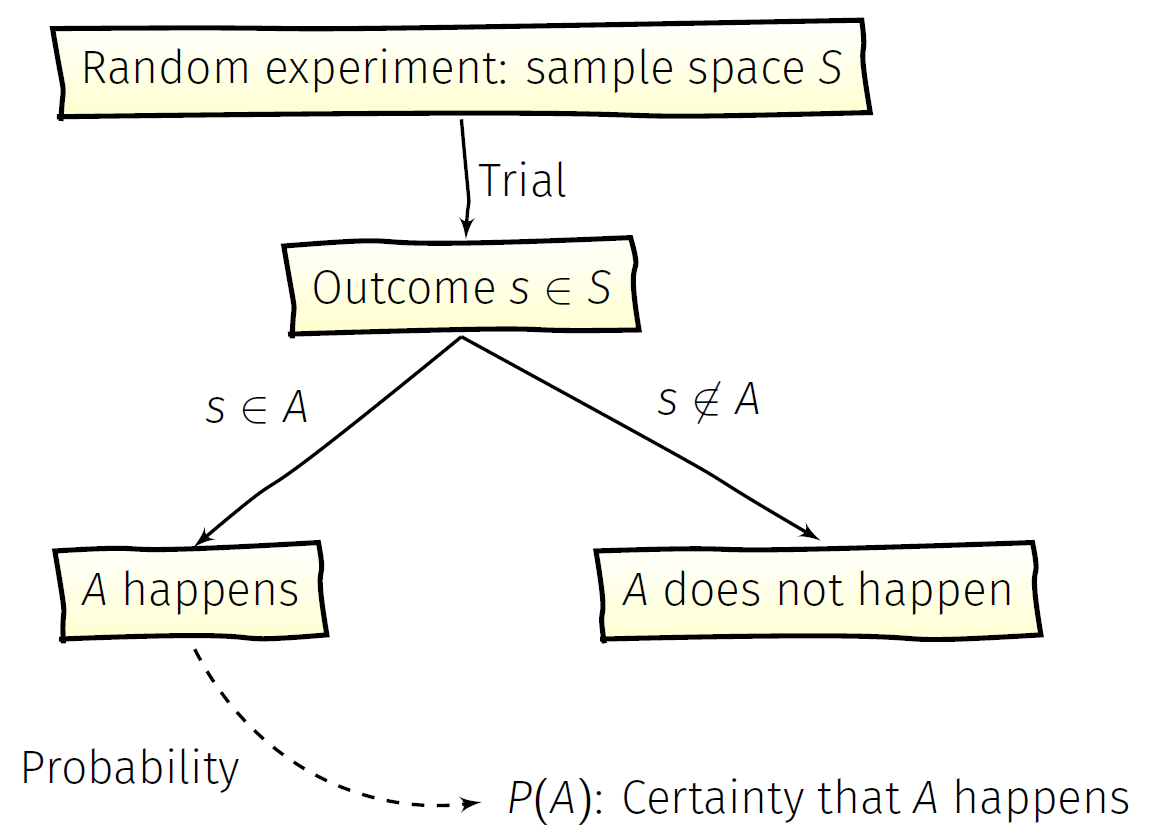
\includegraphics[width=0.65\textwidth]{figs/1_review_prob_intuition.PNG}
    \caption{Intuition of probability. Figure obtained from \cite{psaromiligkos_slides_2019}.}
    \label{fig:prob. intuition}
\end{figure}

\begin{mydefinition}[Probability]
    \emph{Probability} is a set function $\prob{}:\pSet_{S}\mapsto [0,1]$ that assigns to an event $A\in\pSet_{S}$ (recall $A\subseteq S)$ a number $\prob{A}$ that satisfies the following three axioms:
    \begin{enumerate}
        \item $\prob{A}\geq0$,
        \item $\prob{S}=1$, and
        \item For any sequence of mutually exclusive events $A_{1}, A_{2}, \ldots$ (i.e., for which $A_{i}\bigcap A_{j}=\emptyset$ for $i\neq j$), we have
        \begin{align}
            \prob{\bigcup_{i=1}^{\infty} A_{i}}=\sum_{i=1}^{\infty} \prob{A_{i}}.
        \end{align}
    \end{enumerate}
    The number $\prob{A}$ is called the probability of $A$.
\end{mydefinition}
\begin{remark}
        It is NOT always possible to define a function $P:\pSet\mapsto[0,1]$ that satisfies the three axioms.
        Workaround: focus on the events in a $\sigma$-algebra $\fCal$.
        
        Here are some other remarks about the probability function.
        \begin{myBlueBox}
            \begin{itemize}
                \item The probability function $\prob{}:\pSet_{S}\mapsto[0,1]$ maps  the power set $\pSet_{S}$ (or $\sigma$-algebra) to $[0,1]$. That is, the argument of $P$ should be an \emph{element} of $\pSet_{S}$. And since $\pSet_{S}$ is a \emph{set of sets} of $S$, then the argument is the event which is denoted by $\{a_{1},a_{2},\ldots,a_{n}\}=A\in\pSet_{S}$, where $a_{1}, \ldots, a_{n} \in S$.  Thus the proper way to write ``the probability of event $A$'' is $\prob{\{A\}}$ but the notation $\prob{A}$ will often be used for ease of reading and writing.

                \item Note that $\prob{A} = 0$ implies that event $A$ is \emph{improbable}; not necessarily impossible! It's still possible to get $A$. This might be a little unintuitive, but it can be thought of that the chance of $A$ happening is so small that it seems that event $A$ is highly unlikely to occur.
                \item Similarly, $\prob{A}= 1$ does NOT imply that $A$ will certainly occur! It just implies that it is very probably.
            \end{itemize}
        \end{myBlueBox}
\end{remark}

\begin{mydefinition}[$\sigma$-algebra]
    A set $\fCal$ of subsets of $S$, that is, $\fCal\subseteq \pSet$ is \emph{$\sigma$-algebra} if and only if
    \begin{enumerate}
        \item $S\in\fCal$,
        \item $E\in\fCal\implies E^{\comp}\in\fCal$, and
        \item If the sets $A_{1}, A_{2}, \ldots$ belong to $\fCal$, then so does $\bigcup_{i=1}^{\infty}A_{i}$.
    \end{enumerate}
    If $S$ is countable, then $\fCal=\pSet_{S}$ is used.
\end{mydefinition}
A random experiment is modeled as a probability space.
\begin{mydefinition}[Probability space]
    \label{def: proability space}
    A \emph{probability space} is a triplet
    \begin{align}
        (S, \fCal, \prob{}),
    \end{align}
    where
    \begin{enumerate}
        \item $S$: is the sample set,
        \item $\fCal$ is the events algebra, and
        \item $\prob{}:\fCal\mapsto[0,1]$ is the probability function.
    \end{enumerate}
\end{mydefinition}

\section{Basic theorems}
\begin{mytheoremarg}[Basic theorems]
    \label{thm:basic theorems of probability}
    Below is a list of basic theorems of probability.
    \begin{enumerate}
        \item For any event $A\in\fCal$, 
        \begin{align}
            \prob{A^{\comp}} = 1-\prob{A}.
        \end{align}

        \item For any event $A\in\fCal$, 
        \begin{align}
            0\leq \prob{A} \leq 1.
        \end{align} 
        
        \item $\prob{\emptyset} = 0$.
        \item For any events $A, B\in\fCal$, 
        \begin{align}
            \prob{A-B} = \prob{A} - \prob{A\cap B}.
        \end{align}
        Special case: if $B\subseteq A$, then
        \begin{align}
            \prob{A-B} = \prob{A}-\prob{B}.
        \end{align}
        
        \item For any $A, B \in \fCal$, 
        \begin{align}
            \prob{A} = \prob{AB} + \prob{AB^\comp}.
        \end{align}
        
        \item For any $A,B\in\fCal$,
        \begin{align}
            \prob{A\cap B} &= \prob{A} + \prob{B} - \prob{A\cup B},\\
            \prob{A\cup B} &= \prob{A} + \prob{B} - \prob{A\cap B}.
        \end{align}
    \end{enumerate}
\end{mytheoremarg}

\section{Conditional probabilities}
 Events can affect other events. Therefore, the question ``what's the probability of event $A$ happening?'' could be quite different from ``what's the probability of event $A$ \emph{given that event $B$ happened}?''\footnote{In some cases, the two questions are the same. This brings the notion of independence.}. The notation
 \begin{align}
   \prob{A |~ B}    
 \end{align}
reads ``probability of event $A$ happening given that event $B$ happened''.

Given 
\begin{enumerate}
    \item a random experiment $(S, \mc{F}, \prob )$, and
    \item $A, ~B\in\mc{F}$ with $\prob{B}\neq0$.
\end{enumerate}

\begin{mydefinition}
    [Conditional probability]    
    The conditional probability of $A$ given $B$, $\prob{A\middle|~B}$, defined as 
    \begin{align}
        \prob{A|B} &= \f{\prob{A\bigcap B}}{\prob{B}}.
    \end{align}    
\end{mydefinition}
\begin{mytheorem}
  [Conditional probability]    
  Let $B\in\mc{F}$ with $\prob{B}\neq 0$. The mapping 
  \begin{align}
    \prob{\cdot|B}:\mc{F}\to\rnums,
  \end{align}  
  satisfies the axioms of probability
  \begin{enumerate}
      \item $\prob{A|B}\geq 0,\quad \forall A\in\mc{F}$
      \item $\prob{S|B}=1$
      \item If $A_{1}, A_{2},\ldots\in\mc{F}$ is a sequence of mutually exclusive events, then
      \begin{align}
        \prob{\bigcup_{i=1}^{\infty}A_{i}|~B} &= \sum_{i=1}^{\infty}\prob{A_{i}|B}.
      \end{align}
  \end{enumerate}
\end{mytheorem}
Therefore,
\begin{itemize}
    \item For a given event $B$ with $\prob{B}\neq 0$, the mapping
    \begin{align}
        \prob{\cdot | B} : \mc{F}\to\rnums,
    \end{align}
    defines a valid probability function.
    \item All the basic theorems of probability listed in Theorem~\ref{thm:basic theorems of probability}apply to $\prob{\cdot|B}$.
\end{itemize}
\begin{myBlackBox}
    Here are some properties of conditional probability
    \begin{enumerate}
        \item For $A, B \in\mc{F}$ with $\prob{A},\prob{B}\neq0$:
        \begin{align}
            \prob{AB} &= \prob{A|B}\prob{B} \\
            &= \prob{B|A}\prob{A}.
        \end{align}

        
        \item \textbf{Total probability}. Let $B_{1},B_{2},\ldots,B_{n}$ be a partition of $S$, with $\prob{B_{i}}\neq 0,\forall i$:
        \begin{align}
            \prob{A} &= \prob{A|B_{1}}\prob{B_{1}} + \prob{A|B_{2}}\prob{B_{2}} + \ldots + \prob{A|B_{n}}\prob{B_{n}}\\
            &= \sum_{i=1}^{n}\prob{A|B_{i}}\prob{B_{i}}.
        \end{align}
        
        \item \textbf{Bayes rule}. Let $B_{1},B_{2},\ldots,B_{n}$ be a partition of $S$, with $\prob{B_{i}}\neq 0,\forall i$:
        \begin{align}
            \prob{B_{i}|A} &= \f{
                \prob{A|B_{i}}\prob{B_{i}}
            }{
                \sum_{j=1}^{n}\prob{A|B_{j}}\prob{B_{j}}
            }.            
        \end{align}
        Special case for $n=1$:
        \begin{align}
            \prob{B|A} &= \f{\prob{A|B}\prob{B}}{\prob{A}}.
        \end{align}
    \end{enumerate}
\end{myBlackBox}

\begin{mydefinition}
  [Indpendence]    
  \label{def:independence}
  The events $A, B\in\mc{F}$ are called \emph{independent} if 
  \begin{align}
    \underbrace{
      \prob{A|B}=\prob{A}}_{\text{requires } \prob{B}\neq0}
      \text{  or  }
    \underbrace{
        \prob{B|A}=\prob{B}}_{\text{requires } \prob{A}\neq0}
      \text{  or  }    
        \prob{AB}=\prob{A}\prob{B}
  \end{align}
\end{mydefinition}
\begin{mydefinition}
  [Independence (multiple events)]    
  The events $A, B, C\in\mc{F}$ are called \emph{independent} if
  \begin{itemize}
      \item They are independent in pairs, \underline{and}
      \item $\prob{ABC}=\prob{A}\prob{B}\prob{C}$.
  \end{itemize}
\end{mydefinition}
\begin{mydefinition}
  [Conditional independence]    
  Events $A, B\in\mc{F}$ are called \emph{conditionally independent given $C\in\mc{F}$, with $\prob{C}\neq 0$}, if
  \begin{align}
      \prob{AB|C} &= \prob{A|C}\prob{B|C}.
  \end{align}
\end{mydefinition}
\begin{myBlueBox}
    \textbf{Remark:} Conditional independence is quite different from independence. They do not imply each other. Here are some examples.
    
    \begin{example}[Independent but conditionally dependent]
        Two fair coins are flipped. Define the following events
        \begin{itemize}
            \item $A$ - Your first coin flip is heads,
            \item $B$ - Your second coin flip is heads, and
            \item $C$ - Your first two flips were the same.
        \end{itemize}
        Then $A$ and $B$ are independent. However, $A$ and $B$ are conditionally dependent given $C$, since if you know $C$ then your first coin flip will inform the other one.    
    \end{example}
    \begin{example}[Dependent but conditionally independent]
        Consider two brothers John and Joseph, both having a genetic disease. These two events are dependent as they are brothers. However, given the condition that Joseph is an adopted son of the family makes the events independent.
    \end{example}
\end{myBlueBox}

\section{Random variables and distributions}
In many random experiments, it is convenient to assign numerical labels to outcomes.
\begin{example}
    Experiment: pick a car out of a black Escort ($Eb$), a red Escort ($Er$), and a red Mazda ($Mr$).
    The sample space is then 
    \begin{align}
        S = \left\{ Eb, Er, Mr\right\},
    \end{align}
    and the events algebra is $\mc{F}=\pSet$.

    Say we are interested in the make of the car and not the color. Then we can assign labels as can be seen in Figure~\ref{fig:1 assigning numerical labels to outcomes}.
    \begin{figure}[h]
        \centering
        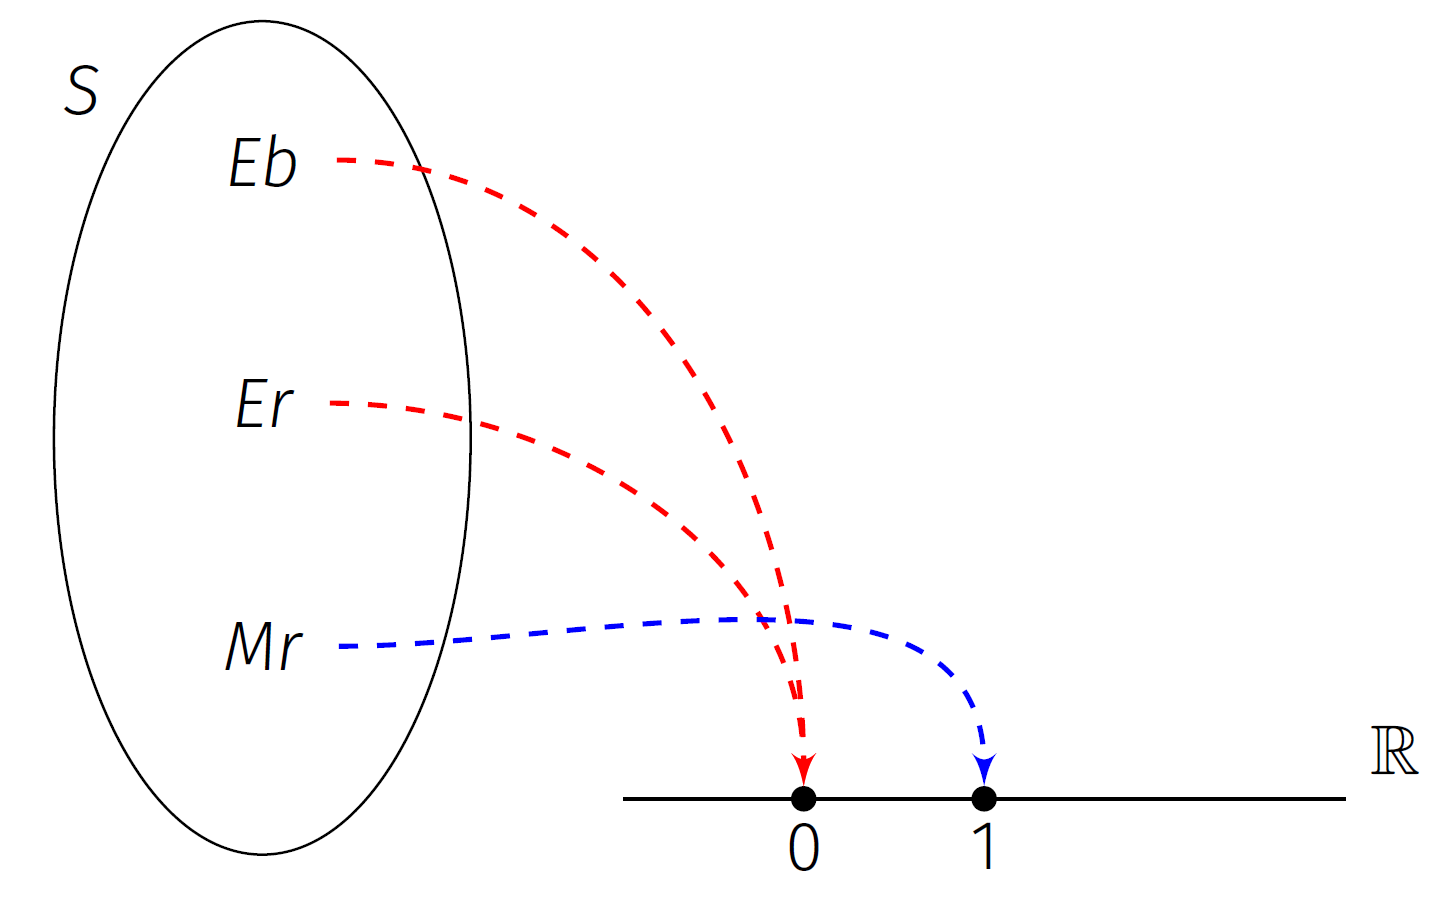
\includegraphics[width=0.65\textwidth]{figs/1_RV_example_labels_car.PNG}    
        \caption{Assigning numerical labels to outcomes; each color is an outcome. From~\cite{psaromiligkos_slides_2019}}
        \label{fig:1 assigning numerical labels to outcomes}
    \end{figure}
\end{example}
\begin{mydefinition}
  [Random variable (RV)]    
  A \emph{random variable (RV)} (denoted by an underline) $\rv{x}:S\to\rnums$ is a mapping from $S$ to $\rnums$ with the following properties.
  \begin{enumerate}
      \item $A(x) = \left\{ s\in S : \rv{x}(s)\leq x\right\}\in\mc{F}, \forall x\in\rnums$
      \item $\prob{\left\{ s\in S: \rv{x}(s)=\infty\right\}}=0$ and $\prob{\left\{ s\in S: \rv{x}(s)=-\infty\right\}}=0$
  \end{enumerate}
  $S$ is referred to as the \emph{domain} of the RV $\rv{x}(\cdot)$ (since a RV is a mapping, then it has a domain and a range). [The domain can be thought of as the sample space\footnote{Not quite sure of this statement.}.]
\end{mydefinition}
\begin{mydefinition}
  [Cumulative distribution function (CDF)]    
  The function $F : \rnums\to[0,1]$ defined by 
  \begin{align}
      F(x) 
      \label{eq:def CDF full}
      &= \prob{s\in S : \rv{x}(s)\leq x}\\
      \label{eq:def CDF shorthand}
      &= \prob{\rv{x}\leq x}, \quad \forall x\in\rnums
  \end{align}
  is called the \emph{cumulative distribution function (CDF)} of $\rv{x}$. Note that \eqref{eq:def CDF shorthand} is a shorthand for \eqref{eq:def CDF full}.

  \textbf{Note:} sometimes the CDF will be denoted with a subscript of the RV (e.g., $F_{x}(x)$). This is for clarity as to make sure that the CDF is over the RV $\rv{x}$. This come more in handy when there are multiple variables in hands (such as in integration).
\end{mydefinition}

\subsection{Properties of random variables}
Here are some properties of random variables.
\begin{enumerate}
    \item $\lim_{x\to\infty} F_{x}(x) =1$ and $\lim_{x\to-\infty} F_{x}(x)=0$
    \item $F_{x}(x)$ is non-decreasing 
    \item $F_{x}(x)$ is continuous from the right. That is
    \begin{align}
        \lim_{x\to x_{0}^{+}} F_{x}(x) &= F_{x}(x_{0})
    \end{align}
    \item $\prob{\left\{ x_{1}<\rv{x}\leq x_{2}\right\}}=F_{x}(x_{2})-F_{x}(x_{1})$
    \item $\prob{\left\{ \rv{x}=x_{1}\right\}}=F_{x}(x_{1})-F_{x}(x_{1}^{-})$, where $F_{x}(x_{1}^{-}):=\lim_{x\to x_{1}^{-}} F_{x}(x)$
    \item $\prob{\left\{ x_{1}\leq \rv{x} \leq x_{2}\right\}}=F_{x}(x_{2})-F_{x}(x_{1}^{-})$
\end{enumerate}

\begin{mydefinition}
  [Types of RVs]    
  A RV $\rv{x}$ is called 
  \begin{itemize}
      \item \emph{Discrete} if $F_{x}(x)$ is constant except of countable number of discontinuities (piecewise constant). Figure~\ref{fig: example CDF discrete RV} shows an example of a CDF of a discrete RV.
      \item \emph{Continuous} if $F_{x}(x)$ is
      \begin{enumerate}
          \item continuous, and
          \item differentiable (with the exception of a countable number of point).
      \end{enumerate}
      \item \emph{Mixed} if it is neither continuous nor discrete.
  \end{itemize}
\end{mydefinition}

\begin{mydefinition}
  [Probability mass function (PMF)]    
  Let $\rv{x}$ be a discrete RV. Then,
  \begin{itemize}
      \item $\prob{\rv{x}=x}=0$ when $x\neq x_{i}, i=1,2,\ldots$, 
      \item $\mc{R}_{x}=\left\{ x_{i} : i=1,,2,\ldots\right\}$ is the set of possible points. 
  \end{itemize}

  The \emph{probability mass function (PMF)} of a RV $\rv{x}$, $\pmf{x}$ or $p_{x}(x)$, $x\in\rnums$, is defined as 
  \begin{align}
      \pmf{x} &= \prob{\rv{x}=x} &= 
      \begin{cases}
          0 & \text{if } x\notin \mc{R}_{x},\\
          \prob{\rv{x}=x_{i}} & \text{if } x\in\mc{R}_{x}, \text{ i.e., } x=x_{i}, i=1,2,\ldots.
      \end{cases}
  \end{align}
  Also,
  \begin{itemize}
      \item $\sum_{i=1}^{\infty}\pmf{x_{i}} = 1$ and $\pmf{x}\geq 0$, $\forall x$ (defining properties),
      \item $\prob{\rv{x}\in \mc{A}}=\sum_{x_{i}\in \mc{A}} \pmf{x_{i}}$.
  \end{itemize}
\end{mydefinition}

\begin{figure}[h]
    \centering
    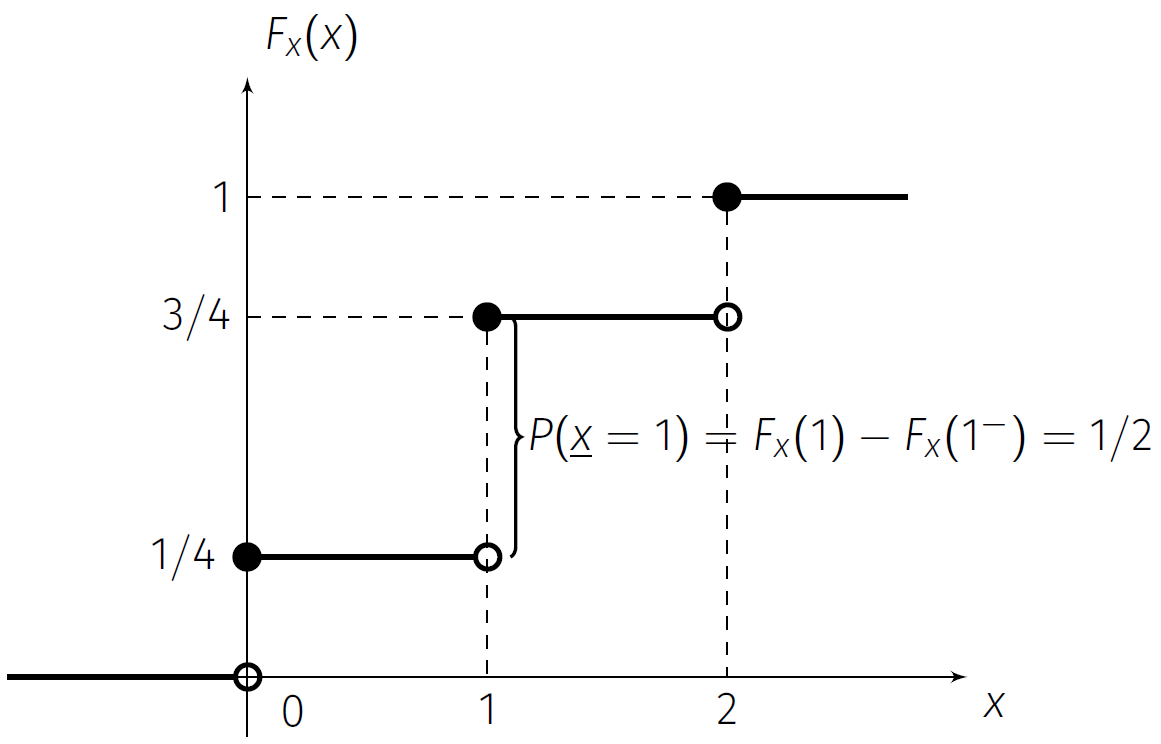
\includegraphics[width=0.65\textwidth]{figs/1_RV_example_discrete.PNG}    
    \caption{Example of a CDF of a discrete RV. From~\cite{psaromiligkos_slides_2019}.}
    \label{fig: example CDF discrete RV}
\end{figure}

\begin{mydefinition}
  [Porbability density function (PDF)]    
  The \emph{probability density function (PDF)}, $\pdf{x}$ or $\pdf{}_{x}(x)$, of a RV $\rv{x}$ is defined as
  \begin{align}
      \pdf{}_{x}(x) &= \td{\cdf{}_{x}(x)}{x}.
  \end{align}
\end{mydefinition}

\subsection{Properties of PDFs}
If $\rv{x}$ is continuous with PDF $\pdf{x}$
\begin{enumerate}
    \item $\pdf{}_{x}(\rv{x})\geq 0, \forall x$ (defining property)
    \item $\int_{-\infty}^{x}\pdf{}_{x}(\lambda)\dee\lambda = \cdf{}_{x}(x)$
    \item $\int_{-\infty}^{\infty}\pdf{}_{x}(x)\dee\lambda = 1$ (defining property)
    \item 
    \begin{align}
        \prob{\left\{ a\leq \rv{x}\leq b\right\}} &= \int_{a}^{b}\pdf{}_{x}(\lambda)\dee\lambda \\
        \prob{\left\{ a< \rv{x}\leq b\right\}} &= \prob{\left\{ a\leq \rv{x}< b\right\}} = \prob{\left\{ a< \rv{x}< b\right\}}.
    \end{align}
\end{enumerate}
\begin{myBlackBox}
    \textbf{Interpretation of PDF}: For a continuous $\rv{x}$: $\prob{\rv{x}=x}=0$ for all $x\in\rnums$ which implies that the PDF $\pdf{x}$ is \emph{not} a probability.

    For small $\epsilon>0$: 
    \begin{align}
        \prob{\abs{\rv{x}-x}<\epsilon} &= \prob{x-\epsilon<\rv{x}<x+\epsilon}\\
        &= \int_{x-\epsilon}^{x+\epsilon}\pdf{t}\dee t\\
        &\approx 2\epsilon\pdf{x}
    \end{align}
    assuming $\pdf{x}$ is continuous at $x$. Equivalently,
    \begin{align}
        \pdf{x}&\approx \f{1}{2\epsilon}\prob{x-\epsilon<\rv{x}<x+\epsilon}.
    \end{align}
    $\pdf{x}$ is proportional to the probability that $\rv{x}$ lies in a small neighbourhood of $x$.
\end{myBlackBox}


\subsection{Conditional distributions}
\begin{mydefinition}[Conditional distributions]      
    \label{def:SRV conitional distributions}
    Let $M\in\mc{F}$ with $\prob{M}\neq 0$. Then
    \begin{enumerate}
        \item \emph{Conditional CDF} of $\rv{x}$ given event $M$ is 
        \begin{align}
            \cdf{}_{x}(x|M) &= \prob{\rv{x}\leq x|M}\\
            &= \f{\prob{\rv{x}\leq x,M}}{\prob{M}}.
        \end{align}
        \item \emph{Conditional PDF} of $\rv{x}$ given event $M$ is
        \begin{align}
            \pdf{}_{x}(x|M) &= \td{\cdf{}_{x}(x|M)}{x}.
        \end{align}
        \item \emph{Conditional PMF} of $\rv{x}$ ($\rv{x}$ discrete given $M$) is
        \begin{align}
            \pmf{x|M} 
            &=
            \begin{cases}
                0, &x \notin\left\{ x_{i} : i = 1,2,\ldots\right\}\\
                \prob{\rv{x}=x_{i}|M}, &x\in\left\{ x_{i} : i=1,2,\ldots\right\}.
            \end{cases}
        \end{align}
        Note that conditional CDFs, PDFs, and PMFs behave like unconditional ones.
    \end{enumerate}
\end{mydefinition}
\subsubsection*{Properties of conditional distributions}
Let $B_{1}, B_{2}, \ldots, B_{n}$ be a partition of $S$, $\prob{B_{i}}\neq 0$. Let $A\in\mc{F}$, $\prob{A}\neq0$.
\begin{itemize}
    \item \textbf{Total probability}:
    \begin{align}
        \cdf{}_{x}(x) &= \sum_{i=1}^{n} \cdf{}_{x}(x|B_{i})\prob{B_{i}},\\
        \pdf{}_{x}(x) &= \sum_{i=1}^{n} \pdf{}_{x}(x|B_{i})\prob{B_{i}},\\
        \pmf{}_{x}(x) &= \sum_{i=1}^{n} \pmf{}_{x}(x|B_{i})\prob{B_{i}}.
    \end{align}
    \item \textbf{Bayes rule}: 
    \begin{align}
        \prob{A|\rv{x}\leq x} 
        &= \f{\prob{\rv{x}\leq x, A}}{\prob{\rv{x}\leq x}}\\
        &= \f{\prob{\rv{x}\leq x|A}\prob{A}}{\prob{\rv{x}\leq x}}\\
        &= \f{\cdf{}_{x}(\rv{x}\leq x|A)\prob{A}}{\cdf{}_{x}({\rv{x}\leq x})}.
    \end{align}
\end{itemize}
When $\rv{x}$ is discrete with $\mc{R}_{x}=\left\{ x_{1},x_{2},\ldots\right\}$, $\pmf{x_{i}}\neq0$:
\begin{itemize}
    \item \textbf{Conditional probability} using PMF:
    \begin{align}
        \prob{A|\rv{x}=x_{i}} 
        &= \f{\prob{A,\rv{x}=x_{i}}}{\prob{\rv{x}=x_{i}}}\\
        &= \f{\prob{A,\rv{x}=x_{i}}}{\pmf{}_{x}({\rv{x}=x_{i}})}.
    \end{align}
    \item \textbf{Total probability}:
    \begin{align}
        \prob{A} &= \sum_{i=1}^{\infty}\prob{A|\rv{x}=x_{i}}\pmf{x_{i}}.
    \end{align}
    \item \textbf{Bayes rule}:
    \begin{align}
        \pmf{x|A} 
        &= \f{\prob{A|\rv{x}=x}\pmf{x}}{\prob{A}}\\
        &= \f{\prob{A|\rv{x}=x}\pmf{x}}{\sum_{i=1}^{\infty}\prob{A|\rv{x}=x_{i}}\prob{x_{i}}}.
    \end{align}
\end{itemize}
When $\rv{x}$ is continuous, it is not possible to divide by $\prob{\rv{x}=x}=0$. Therefore, another definition for conditional PDF is needed.
\begin{mydefinition}
  [Conditional PDF]    
  The \emph{conditional PDF} of $A\in\mc{F}$ given $\rv{x}=x$ (assuming $\pdf{}_{x}(x)\neq0$) is
  \begin{align}
      \prob{A| \rv{x}=x} &= \f{\pdf{}_{x}(x|A)\prob{A}}{\pdf{}_{x}(x)}.
  \end{align}
\end{mydefinition}
The properties of such conditional PDF are
\begin{itemize}
    \item \textbf{Total probability}: $\prob{A}=\int_{-\infty}^{\infty} \prob{A|\rv{x}=x}\pdf{}_{x}(x)\dee x$/
    \item \textbf{Bayes rule}:
    \begin{align}
        \pdf{}_{x}(x|A) 
        &= \f{\prob{A|\rv{x}=x}\pdf{}_{x}(x)}{\prob{A}}\\
        &= \f{\prob{A|\rv{x}=x}\pdf{}_{x}(x)}{\int_{-\infty}^{\infty}\prob{A|\rv{x}=x}\pdf{}_{x}(x)\dee x}.
    \end{align}
\end{itemize}



\section{Transformed random variables}
\label{sec: SRV: Transformed random variables}
Say there exists a random variable $\rv{x}: S\to\rnums$ that is applied on the probability space $(S,\mc{F},\prob{})$. Further, say there exists a [deterministic] function $g:\rnums\to\rnums$. Then, there is a new RV $\rv{y}$ defined as 
\begin{align}
    \rv{y}(s) &= g(\rv{x}(s)) \quad\forall s\in S.
\end{align}
Furthermore, say the distribution (i.e., CDF and PDF (or PMF)) of $\rv{x}$ is known. THen what is the distribution of $\rv{y}=g(\rv{x})$?

The foundation is the following
\begin{align}
    \prob{\rv{y}\in{A}}
    &= \prob{\left\{ s\in S : \rv{y}(s)\in A\right\}}\\
    &= \prob{\left\{ s\in S : g(\rv{x}(s))\in A\right\}}.
\end{align}

There are different methods to find the distribution of a transformed random variable (i.e., $\rv{y}=g(\rv{x})$) depending on the types of variables.
\begin{enumerate}
    \item \textbf{Method of distributions} works when for \emph{any} types of random variables (continuous or discrete). However, it is the most exhaustive method.
    \item \textbf{Method of transformations} works for \emph{continuous} random variables; i.e., both $\rv{x}$ and $\rv{y}$ are continuous.
    \item \textbf{Discrete transformation} for \emph{discrete} transformed variable $\rv{y}$ and \emph{continuous} or \emph{discrete} domain random variable $\rv{x}$.
\end{enumerate}

\subsection{Method of distribution}
The method will be motivated by an example. 
\begin{example}
    Consider the transformed random variable
    \begin{align}
        \rv{y} 
        &= g(\rv{x})\\
        &= \rv{x}^{2}.
    \end{align}
    Evaluate the CDF as follows
    \begin{align}
        \cdf{}_{y}(y) &= \prob{\rv{y}\leq y} = \prob{g(\rv{x})\leq y} = \prob{\rv{x}^2\leq y}\\
        &= \prob{\left\{ s\in S : \rv{x}(s)^{2}\leq y\right\}}.
    \end{align}
    There are three cases
    \begin{enumerate}
        \item $y<0$: $\prob{\rv{x}^{2}\leq y} = 0 \implies \cdf{}_{y}(y) = 0$.
        \item $y=0$: $\prob{\rv{x}^{2}\leq 0} = \prob{\rv{x}^{2}=0} = \prob{\rv{x}=0} \implies \cdf{}_{y}(0)=\prob{\rv{x}=0}$.
        \item $y>0$: $\prob{\rv{x}^{2}\leq y} = \prob{\abs{\rv{x}}\leq \sqrt{y}} = \prob{-\sqrt{y}\leq \rv{x} \leq\sqrt{y}}\implies$
        \begin{align}
            \cdf{}_{y}(y) &= \int_{-\sqrt{y}}^{\sqrt{y}} \pdf{}_{x}(x)\dee x.            
    \end{align}
    \end{enumerate}
\end{example}

\subsection{Method of transformation}
The process is outlined by the following steps. 

\begin{myBlackBox}
    For any $y$ (treat it as a deterministic variable):
    \begin{enumerate}
        \item Solve $g(x)=y$ for $x$. List \emph{all} possible solutions $x_{1},x_{2},\ldots,x_{n}$.
        \item Calculate $g'(x) = \td{g(x)}{x}$.
        \item Evaluate 
        \begin{align}
            \pdf{}_{y}(y) 
            &= 
            \begin{cases}
                0, &\text{no solutions to }g(x)=y,\\
                \sum_{i=1}^{n} \f{\pdf{}_{x}(x_{i})}{\abs{g'(x_{i})}}, &\text{otherwise}.
            \end{cases}
        \end{align}
    \end{enumerate}
\end{myBlackBox}
The method is derived in \cite[Sec.~2.6.2]{murphy_machine_2012}. 

\begin{example}[Method of transformation]
    Consider 
    \begin{align}
        \rv{y} 
        &= g(\rv{x})\\
        &= \rv{x}^{2}.
    \end{align}
    Carry the steps:
    \begin{enumerate}
        \item Solve for $x$ in $y=g(x)$ for all possible cases of $y$:
        \begin{enumerate}
            \item $y<0$: No solutions.
            \item $y=0$: One solution $x_{1}=0$.
            \item $y>0$: Two solutions $x_{1}=-\sqrt{y}$ and $x_{2}=\sqrt{y}$.
        \end{enumerate}
        \item Calculate the derivative of the function
        \begin{align}
            g'(x) &= 2x, \quad \forall x.
        \end{align}
        \item Calculate $\pdf{}_{y}(y)$:
        \begin{enumerate}
            \item $y<0$: $\pdf{}_{y}(y) = 0$.
            \item $y=0$: $\pdf{}_{y}(0)=0$.            
            \item $y>0$: 
            \begin{align}
                \pdf{}_{y}(y) &= \f{\pdf{}_{x}(-\sqrt{y})}{\abs{-2\sqrt{y}}} + \f{\pdf{}_{x}(\sqrt{y})}{\abs{2\sqrt{y}}}\\
                &= \f{1}{2\sqrt{y}}\left[ \pdf{}_{x}(-\sqrt{y}) + \pdf{}_{x}(\sqrt{y}) \right].
            \end{align}
        \end{enumerate}
    \end{enumerate}
    \triqed
\end{example}


\subsection{Discrete transformation}
The method will be motivated by two examples:
\begin{enumerate}
    \item continuous to discrete transformation, and
    \item discrete to discrete transformation.
\end{enumerate}
\begin{example}[Continuous to discrete transformation]
    Let $\rv{x}$ be continuous with $f(x)=0$, $x<0$ and
    \begin{align}
        \rv{y} &= g(\rv{x})\\
        &= \floor{\rv{x}} \quad \text{(floor of $\rv{x}$)}.
    \end{align}
    Then the transformed variable $\rv{y}$ is discrete. I.e., $\mc{R}_{y}=\left\{ 0,1,2,\ldots\right\}$.
    
    The PMF of $\rv{y}$ is then given by 
    \begin{align}
        \pmf{}_{y}(y) 
        &= \prob{\rv{y}=y}\\
        &= \prob{\floor{\rv{x}}=y}\\
        &= \prob{y\leq \rv{x}<y+1}\\
        &= \int_{y}^{y+1}\pdf{}_{x}(x)\dee x, \quad y = 0,1,2,\ldots.
    \end{align}
    \triqed
\end{example}
\begin{example}[Discrete to discrete transformation]
    Let $\rv{x}$ be discrete with $\mc{R}_{x}=\mbb{Z}$, and 
    \begin{align}
        \rv{y}
        &= g(\rv{x})\\
        &= \abs{\rv{x}}.
    \end{align}
    Then $\rv{y}$ is also discrete random variable with $\mc{R}_{y}=\left\{ 0,1,2,\ldots\right\}$.

    The PMF of $\rv{y}$ can then be given by
    \begin{align}
        \pmf{}_{y}(y) &= \prob{\rv{y}=y}\\
        &= \prob{\abs{\rv{x}}=y}\\
        &= \prob{\rv{x}=\pm y}\\
        &= 
        \begin{cases}
            \pmf{}_{x}(0), & y=0,\\
            \pmf{}_{x}(-y)+\pmf{}_{x}(y), & y=1,2,\ldots.
        \end{cases}
    \end{align}
    \triqed
\end{example}

\section{Statistics of random variables}
Sometimes, information about the random variables such as the mean is sought after. Information about a random variables are referred to as the \emph{statistics} of it.
\begin{mydefinition}
  [Expectation operator]    
  \label{def: SRV expectation operator}
  The expectation operator $\expect{\cdot}$ is a functional operator that operates on random variables. Specifically:
  \begin{itemize}
      \item For continuous random variables
      \begin{align}
          \expect{g(\rv{x})}
          &= \int_{-\infty}^{\infty} g(x)\pdf{x}\dee x.
        \end{align}
        \item For discrete random variables 
        \begin{align}
            \expect{g(\rv{x})}
            &= \sum_{-\infty}^{\infty} g(x)\pmf{x}.
        \end{align}
  \end{itemize}
  
\end{mydefinition}

\begin{mydefinition}
  [Mean of a random variable]    
  The mean of a random variable $\rv{x}$, $\mu_{x}$, is defined as
  \begin{align}
      \mu_{x} &= \expect{\rv{x}}      
  \end{align}
  which 
  \begin{itemize}
      \item for continuous random variable 
      \begin{align}
        \mu_{x} &= \expect{\rv{x}}\\
        &= \int_{-\infty}^{\infty}x\pdf{x}\dee x,
      \end{align}
      \item while for discrete random variable
      \begin{align}
        \mu_{x} &= \expect{\rv{x}}\\
        &= \sum_{-\infty}^{\infty}x\pmf{x}.
      \end{align}
  \end{itemize}
  and the conditional mean of $\rv{x}$ given event $M$ is
  \begin{align}
      \expect{\rv{x}|M} &= \int_{-\infty}^{\infty} x\pdf{x|M}\dee x.
  \end{align}
\end{mydefinition}

\subsection*{Properties of the mean}
\begin{itemize}
    \item Mean of $\rv{y}=g(\rv{x})$ is
    \begin{align}
        \expect{\rv{y}} &= \expect{g(\rv{x})}\\
        &= \int_{-\infty}^{\infty}g(x)\pdf{}_{x}(x)\dee x.
    \end{align}
    \item Linear property:
    \begin{align}
        \expect{\sum_{i=1}^{n}\alpha_{i}g_{i}(\rv{x})} &= \sum_{i=1}^{n}\alpha_{i}\expect{g_{i}(\rv{x})}.
    \end{align}
    Note that in general,
    \begin{align}
        \expect{g(\rv{x})} \neq g(\expect{\rv{x}}).
    \end{align}
\end{itemize}

\begin{mydefinition}
  [Variance and standard deviation]    
  Let $\rv{x}$ be a random variable. Then the \emph{variance} of $\rv{x}$, $\var{\rv{x}}$, is defined as
  \begin{align}
      \var{\rv{x}} &= \sigma_{x}^{2}\\
      &= \expect{\left(\rv{x}-\expect{\rv{x}}\right)^2}\\
      &= \expect{\rv{x}^2} - \expect{\rv{x}}^2.
  \end{align}
  The \emph{standard deviation} of $\rv{x}$ is $\sigma_{x} = \sqrt{\var{\rv{x}}}$.

  A useful property of the variance is
  \begin{align}
      \var{a\rv{x}+b} &= a^2\var{\rv{x}}.
  \end{align}
\end{mydefinition}

\begin{mytheorem}[Markov's inequality]
    Let $\rv{x}$ be a non-negative random variable. That is, $\prob{\rv{x}<0}=0$. For any $\epsilon>0$:
    \begin{align}
        \prob{\rv{x}\geq \epsilon} \leq \f{\expect{\rv{x}}}{\epsilon}.
    \end{align}
\end{mytheorem}

\begin{mytheorem}[Chebyshev's inequality]
    Let $\rv{x}$ be a random variable with mean $\mu$ and variance $\sigma^2$. Then, for any $\epsilon>0$:
    \begin{align}
        \prob{\abs{\rv{x}-\mu}\geq \epsilon} \leq \f{\sigma^2}{\epsilon}.
    \end{align}
\end{mytheorem}

\begin{mytheorem}[Jensen's inequality]
    Let $g(\cdot)$ be a convex function. Then, 
    \begin{align}
        \expect{g(\rv{x})} \geq g(\expect{\rv{x}}).
    \end{align}
\end{mytheorem}

\subsection{Moments}

\begin{mydefinition}[Moments] 
    The different moments of a random variable are defined as follows.   
    \begin{itemize}
        \item \emph{$n$-th moment} of $\rv{x}$: $m_{n}=\expect{\rv{x}^{n}}$.
        \item \emph{$n$-th central moment} of $\rv{x}$: $\mu_{n}=\expect{(\rv{x}-\expect{\rv{x}})^{n}}$.
        \item \emph{$n$-th absolute moment} of $\rv{x}$: $\expect{\abs{\rv{x}}^{n}}$.
        \item \emph{$n$-th absolute central moment} of $\rv{x}$: $\mu_{n}=\expect{\abs{\rv{x}-\expect{\rv{x}}}^{n}}$.
    \end{itemize}
\end{mydefinition}

\subsection{Characteristic functions}
\begin{mydefinition}
  [Characteristic function]    
  The \emph{characteristic function} of a random variable $\rv{x}$ is the Fourier transform of its PDF. Specifically,
  \begin{align}
      \Phi_{x}(\omega) &= \int_{-\infty}^{\infty} e^{\jmath \omega x}\pdf{}_{x}(x)\dee x,
  \end{align}
  where the inverse expression is given by
  \begin{align}
      \pdf{}_{x}(x) &= \f{1}{2\pi}\int_{-\infty}^{\infty} e^{-\jmath\omega x}\Phi_{x}(\omega) \dee \omega.
  \end{align}
\end{mydefinition}
\begin{mydefinition}
  [Moment generating function]    
  The \emph{moment generating function} of $\rv{x}$ is the Laplace transform of its PDF. Specifically, 
  \begin{align}
      \bar{\Phi}_{x}(s) &= \int_{-\infty}^{\infty} e^{Sx}\pdf{}_{x}(x)\dee x.
  \end{align}
\end{mydefinition}

\begin{mytheorem}[Moment theorem]
    \begin{align}
        \expect{\rv{x}^{n}} &= \left.\f{\dee^{n}}{\dee s^{n}}\bar{\Phi}_{x}\right|_{s=0} 
        = \left.\f{1}{\jmath^{n}}\f{\dee ^{n}}{\dee\omega^{n}}\Phi_{x}(\omega)\right|_{\omega=0}.
    \end{align}
\end{mytheorem}
% \clearpage
% \clearpage
% %%%%%%%%%%%%%%%%%%
% %%%%%%%%%%%%%%%%%%
% %%%%%%%%%%%%%%%%%%
% %   Old Notes
% %%%%%%%%%%%%%%%%%%
% %%%%%%%%%%%%%%%%%%

% \begin{itemize}
%     \item Definitions in slides.
%     \item Probability of an \textit{event}.
%     \item Event: 1,2,3,...,10 (even number could be an event).
%     \item Power set could. \eg, ((H,T),(H),(T),null-set).
%     \item Understand the definition of the event before interpreting the number/probability.
%     \item 
% \end{itemize}

% \begin{itemize}
%     % \item Probability is a measure of an \textit{outcome} ! Not an event!
    
%     \item Note that $P(A) = 0$ implies that event $A$ is \textit{improbable} and NOT impossible! It's still possible to get $A$. This might be a little unintuitive, but it can be thought of that the chance of $A$ happening is so small that it seems that it is highly unlikely to happen.
%     \item Similarly, $P(A) = 1$ does NOT imply that $A$ will occur! It just implies that it is very probably.
    
%     \item A random experiment is modelled as a probability space.
% \end{itemize}


% \subsection{Definitions}
% \begin{itemize}
%     \item A \textbf{probability} is a measure of our certainty or belief that a statement is true. Another definition is ``a probability is how frequently an event will occur''.
    
%     \item A \textbf{random experiment} is an experiment (or physical process) whose outcome is not certain but all of its \textit{possible} outcomes are known and predictable in advance.
    
%     \item The \textbf{sample space} $S$ is the set of all possible outcomes.
    
%     \item The \textbf{event} $A$ is a subset of $S$.
    
%     \item The \textbf{power set} of $S$ is the set containing all subsets of a set $S$.
%     \begin{itemize}
%         \item Notation: $\pSet_S$ or simply $\pSet$.
%         \item $\pSet$ : Set of all events.
%         \item Special events:
%         \begin{itemize}
%             \item $\emptyset \subseteq S$: Impossible event. ($\emptyset$ is the empty set.)
%             \item $S \subseteq S$: Certain event.
%         \end{itemize}
%     \end{itemize}
    
%     \item \textbf{Probability} is a \textit{set function} $P(\cdot)$ ($P:\pSet_{{S}}\mapsto\mathbb{R}$) that assigns an event $A\subseteq S$ a number $P(A)$ that satisfies the following three axioms:
%     \begin{enumerate}
%         \item $P(A) \geq 0$;
%         \item $P(S) = 1$;
%         \item For any sequence of mutually exclusive events $A_1, A_2, \dots$ (\ie, for which $A_i\cap A_j=\emptyset$ if $i\neq j$), then we have $$ P\left(\bigcap_{i=1}^{\infty}A_i\right) = \sum_{i=1}^{\infty}P(A_i).$$
%     \end{enumerate}
    
%     The number $P(A)$ is called the probability of $A$.
    
%     Remarks:
%     \begin{itemize}
%         \item We cannot \textit{always} define a function $P(\cdot)$ that satisfies the 3 axioms.
%         \item Workaround: focus on the events in a $\sigma-$algebra $\fCal$.
%     \end{itemize}
    
%     \item A set $\fCal$ of subsets of $S$ (\ie, $\fCal\subseteq\pSet_S$) is \textit{$\sigma-$algebra} if and only if 
%     \begin{enumerate}
%         \item $S\in\fCal$,
%         \item $E\in\fCal\implies E^{\comp}\in\fCal$, and
%         \item if the sets $A_i\in\fCal~\forall i\in\mathbb{N}_{+} \implies \bigcup_{i=1}^{\infty}A_i \in \fCal$.
%     \end{enumerate}
    
%     If $S$ is countable, then $\fCal = \pSet_S$ is used.
    
%     \item A \textbf{probability}
%     \footnote{Another definition based off $\sigma-$algebra.}
%     is a set function $P\colon\fCal\mapsto\mathbb{R}$ that assigns to an event $A\in\fCal$ a number $P(A)$ that satisfies the following three axioms:
%     \begin{enumerate}
%         \item $P(A) \geq 0$;
%         \item $P(S) = 1$;
%         \item For any sequence of mutually exclusive events $A_i\in\fCal~\forall i\in\mathbb{N}_{+}$ (\ie, for which $A_i\cap A_j=\emptyset$ if $i\neq j$), then we have $$ P\left(\bigcap_{i=1}^{\infty}A_i\right) = \sum_{i=1}^{\infty}P(A_i).$$
%     \end{enumerate}
    
%     The number $P(A)$ is called the probability of $A$.
    
%     \item A \textbf{probability space} is a triplet $\left(S, \fCal, \pSet\right)$.  Where $S$ is the sample space, $\fCal$ is the events algebra, and $P\colon\fCal\mapsto\mathcal{R}$ is the probability function.
% \end{itemize}


% \subsection{Theorems}
% \begin{enumerate}
%     \item $P(A) = 1-P(A^{\comp})$.
%     \item $0\leq P(A) \leq 1$.
%     \item $P(\emptyset) = 0$.
%     \item $P(A-B) = P(A) - P(A\cap B)$. Special case, if $B\subseteq A$, then $P(A-B) = P(A)-P(B)$.
    
%     \item For any $A, B \in \pCal$, $P(A) = P(AB) + P(AB^\comp)$.
    
%     \item For any $A,B\in\fCal$,
%     \begin{itemize}
%         \item $P(A\cap B)  = P(A) + P(B) - P(A\cup B)$, and 
%         \item $P(A\cup B) = P(A) + P(B) - P(A\cap B)$.
%     \end{itemize}
% \end{enumerate}

% %%%%%%%%%%%%%%%%%%%%%%%%%%%%%%%%%%%%




% \clearpage
% \section{Properties}
% Given a random experiment: $(S,\fCal, P)$. Then the conditional probability of event $A$ happening given that event $B$ happened is formally written as $P(A|B)$ and assuming $P(B) \neq 0$, $P(A|B)$ is given by
% \begin{equation*}
%     P(A|B) = \frac{P(A\cap B)}{P(B)}.
% \end{equation*}

% A useful form for $P(A) \neq 0$ and $P(B) \neq 0$ is 

% Useful properties
% \begin{itemize}
%     \item 
%     \begin{equation}
%         P(AB) = P(A|B)P(B) = P(B|A)P(A).    
%     \end{equation}
    
%     \item \textbf{Total probability}:
%     Let $B_1, B_2, ...$ be a partition\footnote{A set of grouping that sets \textbf{elements} into non-empty \textbf{subsets} in such a way that every element is matched in exactly one set.} of $S$ with $P(B_i) \neq 0~i=1,\dots,n$, then 
    
%     \begin{enumerate}
%         \item $P(A) = \sum_{i=1}^{n}P(A|B_i)P(B_i)$.
%         \item $$P(B_i|A) = \frac{P(A|B_i)P(B_i)}{\sum_{i=1}^{n}P(A|B_i)P(B_i)}.$$
%     \end{enumerate}
    
% \end{itemize}

% \subsection{Independence}
% Events $A,B \in \pCal$ are two independent events if 
% \begin{enumerate}
%     \item $P(AB) = P(A)P(B)$.
%     \item If $P(B) \neq 0$, $P(A|B) = P(A)$.
%     \item If $P(A) \neq 0$, $P(B|A) = P(B)$.
% \end{enumerate}

% Events $A, B, C \in \fCal$ are independent if 
% \begin{enumerate}
%     \item they're independent in pairs, and
%     \item $P(ABC) = P(A)P(B)P(C)$.
% \end{enumerate}


% %%%%%%%%%%%%%
% \section{Random variables}
% \subsection{Definition}
% A random variable $\underline{x}$ is basically a mapping from events to numbers (assigning numerical labels to outcomes). In mathematical terms, $\underline{x} : S \mapsto \mathbb{R}$ such that
% \begin{enumerate}
%     \item $A(x) = \{s\in S : \underline{x}(s) \neq x\} \in \fCal,~\forall x\in\mathbb{R}$. I.e., all possible outcomes $s\in S$ such that $\underline{x}(s)\leq x \implies A(x)$ is an event.
%     \item 
%     \begin{enumerate}
%         \item $P(\{s\in S : \underline{x}(s) = +\infty\}) = 0$, and
%         \item $P(\{s\in S : \underline{x}(s) = -\infty\}) = 0$.
%     \end{enumerate}
% \end{enumerate}

% Note that in this course, underlines are associated with random variables. So $\underline{x}$ is a random variable while $x$ is a deterministic variable.

% \subsection{Cumulative Distribution Function (CDF)}
% Defined by

% \begin{equation*}
%     F : \mathbb{R} \mapsto [0,1],
% \end{equation*}
% such that

% \begin{equation}
%     \begin{aligned}
%          F(x) &= P(\{s\in S : \underline{x}(s) \leq x\})\\
%               &= P(\underline{x} \leq x).
%     \end{aligned}
% \end{equation}

% The CDF is associated with the distribution of a random variable, so it is good practice to include a subscript of the random variable to the CDF. I.e., $F_x(\cdot)$ is the CDF of the random variable $\underline{x}$.

% \subsubsection{CDF properties}
% \begin{enumerate}
%     \item $\lim_{x\xrightarrow{}\infty}F_x(x) = 1$ and $\lim_{x\xrightarrow{}-\infty}F_x(x) = 0$.
%     \item $F_x$ is non-decreasing.
%     \item $F_x$ is continuous from the right. I.e., $F_x(x_0^+) = F_x(x_0)$.
%     \item $P(\{x_1<\underline{x}\leq x_2\}) = F_x(x_2)-F_x(x_1)$.
%     \item $P(\underline{x}=x_1) = F_x(x_1)-F_x(x_1^-)$.
%     \item $P(\{x_1\leq\underline{x}\leq x_2\}) = F_x(x_2)-F_x(x_1^-)$.
% \end{enumerate}

% \subsubsection{Types of Random Variables}
% \begin{enumerate}
%     \item \textbf{Discrete} if $F_x(x)$ is constant except for countable number of discontinuities (\ie, $F_x$ is a piecewise constant function).
    
%     \item \textbf{Continuous} if $F_x$ is
%     \begin{enumerate}
%         \item continuous, and
%         \item differentiable with the exception of countable number of points.
%     \end{enumerate}
%     \item \textbf{Mixed} if it's not continuous nor discrete (basically it's a mix of both).
% \end{enumerate}

% \subsection{Probability Mass Function (PMF)}
% A PMF $p(x)$ is basically a PDF for discrete random variables and is defined as

% \begin{equation}
%     p(x) =
%     \begin{cases}
%         0 &x\notin \rCal, \\
%         P(\underline{x} = x_i) & x_i\in\rCal.
%     \end{cases}
% \end{equation}

% \subsubsection{PMF properties}
% \begin{enumerate}
%     \item $\sum_{i=1}^{\infty} p(x_i) = 1$ and $p(x) \geq 0$.
%     \item $P(\underline{x}\in A) = \sum_{x_i\in A}p(x_i)$.
% \end{enumerate}

% \subsection{Probability Distribution Function (PDF)}
% Let $\underline{x}$ be a random variable with CDF $F_x(\cdot)$. Then the PDF of $\underline{x}$ $f(x)$ or $f_x(x)$ is defined as
% \begin{equation}
%     f_x(x) = F_x'(x) = \frac{\dee F_x}{\dee x}(x).
% \end{equation}

% \subsubsection{Properties of a PDF}
% A PDF is NOT a probability! It could be thought of as $f_x(x)$ is proportional to the probability that $\underline{x}$ lies in a  small neighbourhood of x. 

% If $\underline{x}$ is a continuous with PDF $f_x(x)$, then
% \begin{enumerate}
%     \item $f_x(x)\geq0 ~\forall x\in\mathbb{R}$,
%     \item $\int_{-\infty}^{x}f_x(\lambda)\dee\lambda = F_x(x)$,
%     \item $\int_{-\infty}^{\infty}f_x(\lambda)\dee\lambda = 1$, and
%     \item $P(\{a\leq\underline{x}\leq b\}) = P(\{a<\underline{x}< b\}) = \int_{b}^{a}f_x(\lambda)\dee\lambda$.
% \end{enumerate}

% \section{Probability distribution transformations}
% Given $\underline{y} = g(\uline{x})$ and the PMF, CDF, or PDF of $\uline{x}$, what's the  PMF, CDF, or PDF of $\uline{y}$? 

% There are different methods of dealing with this. Namely, 

% \begin{enumerate}
%     \item Methods of distribution. This is the most general method as it does not impose any constraints on the variables. 
%     \item Method of transformation. This method works for continuous $\uline{x}$ that map to continuous $\uline{y}$ variables.
%     \item Direct method of evaluation. Works for discrete $\uline{y}$ (continuous or discrete $\uline{x}$).
% \end{enumerate}